Como afirma \citeonline[Pref�cio]{Meyer}, muitos algoritmos de processamento de sinais, como FFT \textit{(Fast Fourier Transform)} e os filtros FIR ou IIR, implementados anteriormente em PDSPs ou em Circuitos Integrados de Aplica��o Especifica ou ASIC \textit{(Application Specific Integrated Circuits)}, agora est�o sendo implementados em FPGAs.

\citeonline{moore}[p.~4] define a FPGA como um dispositivo semicondutor capaz de ser totalmente redefinido ap�s sua fabrica��o, permitindo ao desenvolvedor reconfigurar produtos e fun��es j� implementadas, adaptando o \textit{hardware} a novas fun��es. De forma pr�tica, a FPGA permite uma flexibilidade em um projeto, podendo mudar a forma como ele � implementado, sem a necessidade de se construir um \textit{hardware} novo.

As FPGAs s�o baseadas em unidades l�gicas elementares b�sicas, capazes de se conectar de diferentes formas criando uma variedade de componentes digitais. Na fam�lia de FPGAs \textit{Spartan$^\circledR$-3E}, fabricadas pela empresa \textit{Xilinx$^\circledR$}, as unidades l�gicas elementares b�sicas s�o chamadas de \textit{slices}. Cada \textit{slice} possui 2 conjuntos de 4 entradas e uma sa�da LUTs \textit{(Look Up Table and Flip-Flops/Latches)}, 2 \textit{flip-flops} e sistema de controle compartilhado. Por fim, um conjunto de 4 \textit{slices}
s�o combinados em um bloco l�gico configur�vel (\textit{Configurable Logic Blocks}, CLB) \cite{Meyer}.

O dispositivo escolhido para a implementa��o do algoritmo Radix-2 � o kit 
de desenvolvimento para FPGA denominado \textit{Spartan$^\circledR$-3E} \textit{FPGA Starter Kit Board}, apresentado na figura 3. Tal kit possui uma FPGA XC3S500E, com 1.164 CLBs, 4.656 \textit{slices}, um bloco de RAM de 360 Kbits, 20 multiplicadores dedicados e 232 portas de entrada e sa�da utiliz�veis \cite{xilinx}.

\vspace{5mm}

\begin{figure}[H]
	\centering
	\captionsetup{width=0.8\textwidth, font=footnotesize, textfont=bf}	
	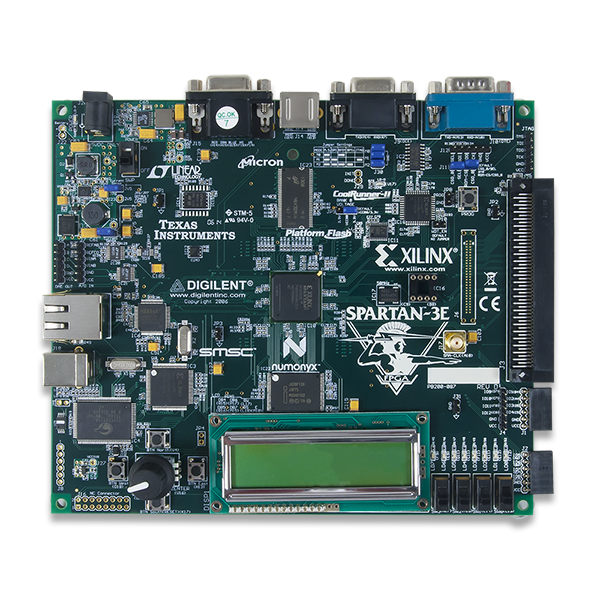
\includegraphics[width=0.8\linewidth]{Images/RevisaoDeLiteratura/spartan-3e.png}
	\caption{\textit{Spartan$^\circledR$-3E FPGA Starter Kit Board}}
	\vspace{-3.5mm}
	\caption*{Fonte: \citeonline{xilinx}}
	\label{fig:FPGA}
\end{figure}

\vspace{5mm}
